\documentclass{article}
\usepackage{listings}
\usepackage{color}
\usepackage{amsmath}
\usepackage{mathtools}
\usepackage{amsfonts}
\usepackage{amssymb}
\usepackage{caption}
\usepackage{tabularx}
\usepackage[export]{adjustbox}
\usepackage{polski}
\usepackage{indentfirst}
\usepackage{graphicx}
\usepackage{pdfpages}
\usepackage{float}
\usepackage{gauss}

\DeclareCaptionType{equ}[][List of equations]
\captionsetup[equ]{labelformat=empty}

%script adding bars in matrix
\usepackage{etoolbox}
\makeatletter
\patchcmd\g@matrix
 {\vbox\bgroup}
 {\vbox\bgroup\normalbaselines}% restore the standard baselineskip
 {}{}
\makeatother

\newcommand{\BAR}{%
  \hspace{-\arraycolsep}%
  \strut\vrule % the `\vrule` is as high and deep as a strut
  \hspace{-\arraycolsep}%
}
\definecolor{dkgreen}{rgb}{0,0.6,0}
\definecolor{gray}{rgb}{0.5,0.5,0.5}
\definecolor{mauve}{rgb}{0.58,0,0.82}

\lstset{frame=tb,
  language=Python,
  aboveskip=3mm,
  belowskip=3mm,
  showstringspaces=false,
  columns=flexible,
  basicstyle={\small\ttfamily},
  numbers=none,
  numberstyle=\tiny\color{gray},
  keywordstyle=\color{blue},
  commentstyle=\color{dkgreen},
  stringstyle=\color{mauve},
  breaklines=true,
  breakatwhitespace=true,
  tabsize=3,
  extendedchars=\true,
  inputencoding=utf8x
}

\lstset{literate={ą}{{\k{a}}}1 {ł}{{\l{}}}1 {ń}{{\'n}}1 {ę}{{\k{e}}}1 {ś}{{\'s}}1 {ż}{{\.z}}1 {ó}{{\'o}}1 {ź}{{\'z}}1 {Ą}{{\k{A}}}1 {Ł}{{\L{}}}1 {Ń}{{\'N}}1 {Ę}{{\k{E}}}1 {Ś}{{\'S}}1 {Ż}{{\.Z}}1 {Ó}{{\'O}}1 {Ź}{{\'Z}}1 }

\begin{document}
\title{Sprawozdanie - Metody numeryczne i optymailzacja}
\author{Jakub Andryszczak 259519,\\ Jakub Żak 244255,\\ Maciej Cierpisz 249163}
\date{}
\maketitle

\newpage
\tableofcontents
%Tutaj zaczyna się wstęp

\newpage
\section{Zadanie nr. 1}
Znajdź zmienne \(x_1\) oraz \(x_2\), które minimalizują funkcję celu \(x_1 + x_2\) przy ograniczeniu:
\[
x_1^2 + x_2^2 = 2.
\]

Aby rozwiązać podane zadanie optymalizacji, użyjemy metody mnożników Lagrange'a. Zadanie polega na znalezieniu zmiennych \(x_1\) oraz \(x_2\), które minimalizują funkcję celu \(f(x_1, x_2) = x_1 + x_2\) przy ograniczeniu \(g(x_1, x_2) = x_1^2 + x_2^2 - 2 = 0\).

Metoda mnożników Lagrange'a polega na wprowadzeniu nowej zmiennej \(\lambda\) (mnożnika Lagrange'a) i rozwiązaniu układu równań danych przez gradienty funkcji Lagrange'a:
\[ \nabla f = \lambda \nabla g \]

Funkcja Lagrange'a jest zdefiniowana jako:
\[ \mathcal{L}(x_1, x_2, \lambda) = f(x_1, x_2) + \lambda (g(x_1, x_2)) \]
\[ \mathcal{L}(x_1, x_2, \lambda) = (x_1 + x_2) + \lambda (x_1^2 + x_2^2 - 2) \]

Teraz obliczamy pochodne cząstkowe i przyrównujemy je do zera:
\[ \frac{\partial \mathcal{L}}{\partial x_1} = 1 + \lambda \cdot 2x_1 = 0 \]
\[ \frac{\partial \mathcal{L}}{\partial x_2} = 1 + \lambda \cdot 2x_2 = 0 \]
\[ \frac{\partial \mathcal{L}}{\partial \lambda} = x_1^2 + x_2^2 - 2 = 0 \]

Rozwiązując te równania krok po kroku:

1. Z równania \(\frac{\partial \mathcal{L}}{\partial x_1} = 0\):
\[ 1 + 2\lambda x_1 = 0 \]
\[ \lambda = -\frac{1}{2x_1} \]

2. Z równania \(\frac{\partial \mathcal{L}}{\partial x_2} = 0\):
\[ 1 + 2\lambda x_2 = 0 \]
\[ \lambda = -\frac{1}{2x_2} \]

3. Przyrównując dwa wyrażenia dla \(\lambda\):
\[ -\frac{1}{2x_1} = -\frac{1}{2x_2} \]
\[ x_1 = x_2 \]

4. Używając ograniczenia \(x_1^2 + x_2^2 = 2\):
\[ x_1^2 + x_1^2 = 2 \]
\[ 2x_1^2 = 2 \]
\[ x_1^2 = 1 \]
\[ x_1 = \pm 1 \]

W związku z tym, \(x_2\) również jest \( \pm 1 \). To daje nam dwa punkty:
\[ (x_1, x_2) = (1, 1) \quad \text{lub} \quad (-1, -1) \]

Teraz obliczamy wartość funkcji celu w tych punktach:
\[ f(1, 1) = 1 + 1 = 2 \]
\[ f(-1, -1) = -1 - 1 = -2 \]

Tak więc, minimalna wartość funkcji celu \(x_1 + x_2\) przy danym ograniczeniu jest osiągana w punkcie \((x_1, x_2) = (-1, -1)\).

Zatem zmienne \(x_1\) oraz \(x_2\), które minimalizują funkcję celu to:
\[ x_1 = -1, \quad x_2 = -1 \]

\begin{figure}[h]
    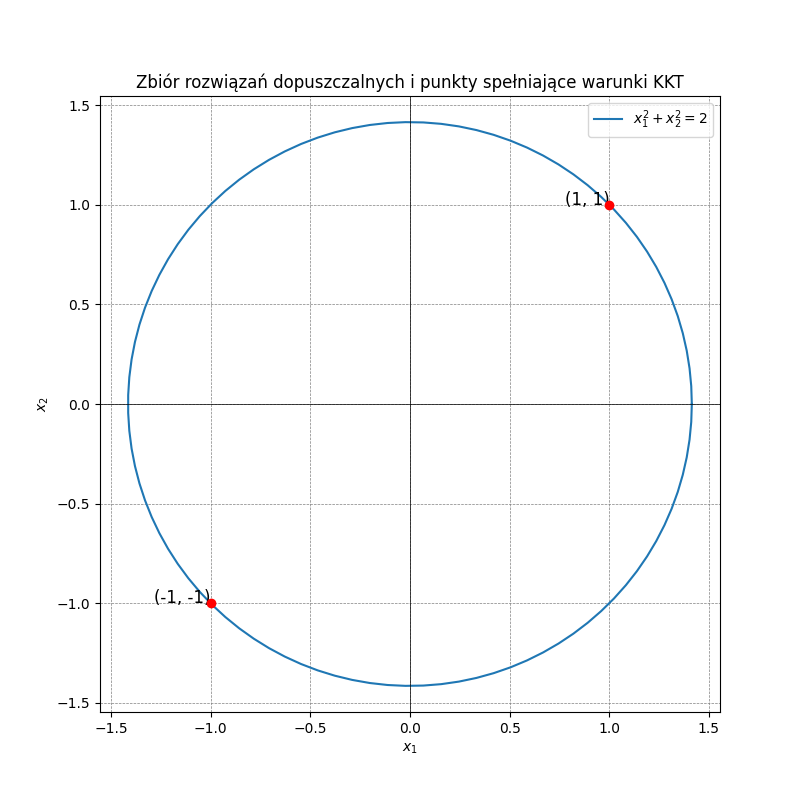
\includegraphics[scale=0.4]{zadanie1.png}
    \title{\newline Rys. 1.1. Wykres dopuszczalnych rozwiązań oraz punktów spełniających warunki optymalności KKT}
    \centering
  \end{figure}
\newpage
\section{Zadanie nr. 2}
Znajdź zmienne \(x_1\) oraz \(x_2\), które minimalizują funkcję celu \(x_1 + x_2\) przy ograniczeniach:
\[
x_2 \geq 0,
\]
\[
2 - x_1^2 - x_2^2 \geq 0.
\]
Narysuj zbiór rozwiązań dopuszczalnych na płaszczyźnie \(\mathbb{R}^2\) i znajdź punkty spełniające warunki optymalności KKT. Które ograniczenia są aktywne? Zilustruj zadanie geometrycznie.
Minimalizujemy funkcję celu:
\[
f(x_1, x_2) = x_1 + x_2
\]
przy ograniczeniach:
\[
g_1(x_1, x_2) = x_2 \geq 0,
\]
\[
g_2(x_1, x_2) = 2 - x_1^2 - x_2^2 \geq 0.
\]

Definiujemy funkcję Lagrange'a:
\[
\mathcal{L}(x_1, x_2, \lambda_1, \lambda_2) = x_1 + x_2 + \lambda_1 (-x_2) + \lambda_2 (2 - x_1^2 - x_2^2)
\]

Gradient funkcji Lagrange'a:
\[
\nabla \mathcal{L} = \left( 1 - 2\lambda_2 x_1, 1 - \lambda_1 - 2\lambda_2 x_2, -x_2, 2 - x_1^2 - x_2^2 \right)
\]

Warunki KKT:
\[
1 - 2\lambda_2 x_1 = 0,
\]
\[
1 - \lambda_1 - 2\lambda_2 x_2 = 0,
\]
\[
\lambda_1 \geq 0, \quad \lambda_1 x_2 = 0,
\]
\[
\lambda_2 \geq 0, \quad \lambda_2 (2 - x_1^2 - x_2^2) = 0.
\]
Rozwiązywanie układu równań

\[
1 - 2\lambda_2 x_1 = 0 \implies \lambda_2 = \frac{1}{2x_1},
\]
\[
1 - \lambda_1 - 2\lambda_2 x_2 = 0 \implies 1 - \lambda_1 - \frac{x_2}{x_1} = 0,
\]

\[
x_1^2 + x_2^2 = 2.
\]
Sprawdzanie ograniczeń aktywnych

- Jeśli \(\lambda_1 = 0\), \(x_2 \geq 0\).
- Jeśli \(\lambda_2 = 0\), \(x_1^2 + x_2^2 = 2\).
Rozwiązanie dla punktów aktywnych

- \(x_1 = -\sqrt{2}\), \(x_2 = 0\),
- \(x_1 = \sqrt{2}\), \(x_2 = 0\).

Minimalizacja funkcji celu

\[
f(-\sqrt{2}, 0) = -\sqrt{2} + 0 = -\sqrt{2},
\]
\[
f(\sqrt{2}, 0) = \sqrt{2} + 0 = \sqrt{2}.
\]

Minimalna wartość funkcji celu jest osiągana w punkcie \((- \sqrt{2}, 0)\).
\begin{figure}[h]
    \includegraphics[scale=0.4]{zadanie2.png}
    \title{\newline Rys. 2.1. Wykres dopuszczalnych rozwiązań oraz punktów spełniających warunki optymalności KKT}
    \centering
  \end{figure}
\newpage
\section{Zadanie nr. 3}
Znajdź zmienne \(x_1\) oraz \(x_2\), które minimalizują funkcję celu \(x_1^2 + x_2^2\) przy ograniczeniu:
\[
x_1 + x_2 \geq 1.
\]
Znajdź rozwiązanie i wykaż, że funkcja celu dla tego rozwiązania ma punkt przegięcia.

Minimalizujemy funkcję celu:
\[
f(x_1, x_2) = x_1^2 + x_2^2
\]
przy ograniczeniu:
\[
g(x_1, x_2) = x_1 + x_2 - 1 \geq 0.
\]

Definiujemy funkcję Lagrange'a:
\[
\mathcal{L}(x_1, x_2, \lambda) = x_1^2 + x_2^2 + \lambda (1 - x_1 - x_2)
\]

Gradient funkcji Lagrange'a:
\[
\nabla \mathcal{L} = \left( 2x_1 - \lambda, 2x_2 - \lambda, 1 - x_1 - x_2 \right)
\]

Warunki KKT:
\[
2x_1 - \lambda = 0, \quad 2x_2 - \lambda = 0, \quad 1 - x_1 - x_2 \geq 0, \quad \lambda \geq 0, \quad \lambda (1 - x_1 - x_2) = 0
\]

Z pierwszych dwóch równań mamy:
\[
2x_1 = \lambda \quad \text{i} \quad 2x_2 = \lambda \implies 2x_1 = 2x_2 \implies x_1 = x_2
\]

Podstawiamy \( x_1 = x_2 \) do ograniczenia:
\[
x_1 + x_1 = 2x_1 \geq 1 \implies x_1 \geq \frac{1}{2}
\]

Zatem \( x_1 = x_2 = \frac{1}{2} \) i \(\lambda = 2x_1 = 1\).


Minimalizowana funkcja celu przyjmuje wartość:
\[
f\left(\frac{1}{2}, \frac{1}{2}\right) = \left(\frac{1}{2}\right)^2 + \left(\frac{1}{2}\right)^2 = \frac{1}{4} + \frac{1}{4} = \frac{1}{2}
\]


Aby wykazać, że funkcja celu ma punkt przegięcia w \( \left( \frac{1}{2}, \frac{1}{2} \right) \), sprawdzimy drugie pochodne funkcji celu:
\[
f(x_1, x_2) = x_1^2 + x_2^2
\]

Drugie pochodne:
\[
\frac{\partial^2 f}{\partial x_1^2} = 2, \quad \frac{\partial^2 f}{\partial x_2^2} = 2, \quad \frac{\partial^2 f}{\partial x_1 \partial x_2} = 0
\]

Macierz Hessego:
\[
H = \begin{bmatrix}
2 & 0 \\
0 & 2
\end{bmatrix}
\]

Wyznacznik macierzy Hessego:
\[
\det(H) = 2 \times 2 - 0 \times 0 = 4 > 0
\]

Ponieważ wyznacznik macierzy Hessego jest dodatni i drugie pochodne są dodatnie, funkcja \( f(x_1, x_2) \) ma minimum w punkcie \( \left( \frac{1}{2}, \frac{1}{2} \right) \). Jest to punkt przegięcia, co można zilustrować geometrycznie.

\section{Zadanie nr. 4}

Rozwiąż następujące zadanie programowania kwadratowego:


\begin{align*}
\min \, \frac{1}{2}x^TQx + c^Tx \\
\text{przy ograniczeniach:} \\
Ax \ge b, \\
x \ge 0,
\end{align*}

Sformułuj zadanie dualne dla powyższego problem. Następnie rozwiąż poniższe zadanie:

\begin{align*}
    \min &\qquad \frac{1}{2}x_1^2 + x_2^2 - x_1x_2 - 2x_1 - 6x_2 \\
    \text{p.o.} &\qquad x_1 + x_2 \leq 2, \\
    &\qquad -x_1 + 2x_2 \leq 2, \\
    &\qquad 2x_1 + x_2^2 \leq 2, \\
    &\qquad x_1 \geq 0, \\
    &\qquad x_2 \geq 0.
    \end{align*}
    
Poniżej kod realizujący zadanie:

\begin{lstlisting}
    import cvxpy as cp

# Zdefiniowane zmienne
x1 = cp.Variable()
x2 = cp.Variable()

# Funkcja celu (do zminimalizowania)
objective = cp.Minimize(x1**2 + x2**2 - 4*x1 - 2*x2 - 6)

# Ograniczenia
constraints = [x1 + x2 <= 2, -x1 + 2*x2 <= 2, 2*x1 + x2 <= 2, x1 >= 0, x2 >= 0]

# Problem programowania kwadratowego
prob = cp.Problem(objective, constraints)

# Rozwiązanie problemu
prob.solve()

# Wyświetlenie wyników
print("Wartość minimalna funkcji:", prob.value)
print("x1:", x1.value)
print("x2:", x2.value)

\end{lstlisting}

Wyniki:
\begin{equation}
    \begin{cases}
        min. funkcji = -9.2\\
        x1 = 0.7999999999999999\\
        x2 = 0.39999999999999997
    \end{cases}
\end{equation}

\section{Zadanie nr. 5}

Rozwiąż zadanie:\\
\begin{align*}
    \min &\qquad x_1^2 + x_2^2 + x_3^2 \\
    \text{p.o.} &\qquad x_1 + 2x_2 - x_3 = 4, \\
    &\qquad x_1 -x_2 +x_3 = -2.
    \end{align*}


Kod realizujący zadanie:
\begin{lstlisting}
    
    import cvxpy as cp

    # Definiowanie zmiennych
    x1 = cp.Variable()
    x2 = cp.Variable()
    x3 = cp.Variable()
    
    # Funkcja celu
    objective = cp.Minimize(x1**2 + x2**2 + x3**2)
    
    # Ograniczenia
    constraints = [
        x1 + 2*x2 - x3 == 4,
        x1 - x2 + x3 == -2
    ]
    
    # Definiowanie problemu
    problem = cp.Problem(objective, constraints)
    
    # Rozwiązywanie problemu
    problem.solve()
    
    # Wyświetlanie wyników
    print("Optymalne wartości zmiennych:")
    print("x1 =", x1.value)
    print("x2 =", x2.value)
    print("x3 =", x3.value)
    print("Minimalna wartość funkcji celu =", problem.value)
    

\end{lstlisting}

Wyniki:
\begin{equation}
    \begin{cases}
        x1=0.28571428571428564\\
        x2=1.4285714285714284\\
        x3=-0.8571428571428571
    \end{cases}
\end{equation}

Minimalna wrtość funkcji celu = 2.8571428571428568.
\section{Zadanie nr. 6}

Rozwiąż zadanie:\\
\begin{align*}
    \min &\qquad x_1^2 - x_2^2 \\
    \text{p.o.} &\qquad x_1 + 2x_2 \geq 2, \\
    &\qquad -5x_1 +4x_2 \leq 10,\\
    &\qquad x_1 \leq 0, \\
    &\qquad x_2 \geq 0.
    \end{align*}

Kod realizujący zadanie: 

\begin{lstlisting}
    
    from scipy.optimize import minimize
    import numpy as np
    
    # Define the objective function
    def objective(x):
        return x[0]**2 - x[1]**2
    
    # Define the constraints
    def constraint1(x):
        return x[0] + 2*x[1] - 2
    
    def constraint2(x):
        return -5*x[0] + 4*x[1] - 10
    
    # Define the bounds manually since COBYLA doesn't support bounds directly
    def cobyla_bounds(x):
        return [x[0], -x[0], x[1]]
    
    # Define the initial guess
    x0 = [-0.1, 1.0]  # Feasible initial guess
    
    # Define the constraints dictionary
    cons = [{'type': 'ineq', 'fun': constraint1},
            {'type': 'ineq', 'fun': constraint2},
            {'type': 'ineq', 'fun': lambda x: x[0]},    # x1 <= 0 --> x1 is negative
            {'type': 'ineq', 'fun': lambda x: x[1]}]    # x2 >= 0 --> x2 is positive
    
    # Solve the problem
    solution = minimize(objective, x0, method='COBYLA', constraints=cons)
    
    # Print the results
    print(f"Optimal value: {solution.fun}")
    print(f"Optimal x1: {solution.x[0]}")
    print(f"Optimal x2: {solution.x[1]}")

\end{lstlisting}

Wyniki:

\begin{equation}
    \begin{cases}
        x1=9.038781217079983\\
        x2=974.2149836274926
    \end{cases}
\end{equation}
Optymalna wartość: -949013.1347584255
\section{Zadanie nr. 7}

\end{document}